Second generation neural networks achieve impressive results
on all tasks that can collectively be identified as data classification.
As of the time of writing, second generation convolutional networks
continue dominating every ImageNet classification challenge of the last
years~\cite{ILSVRC15}.

There are still types of tasks however that no deep learning topology or 
technique has been able to tackle so far. Adversarial evaluations of reading comprehension
systems indicate that neural networks that excell at evaluating carefully
prepared data prove to be extremely fragile when encountering organic ``noise''
information~\cite{DBLP:journals/corr/JiaL17}.
The practice of splitting learning into separate training and application steps
means that a traditional neural network is unable to continuously learn while working.
This way, new information cannot be aquired dynamically as it has to be spoon-fed in the
form of carefully prepared test data.
Further limitations of current deep learning strategies have been compiled by 
Gary Marcus~\cite{DBLP:journals/corr/abs-1801-00631}.

One way to interpret these limitations is as an expression of the growing discrepancy between
biological neural networks and the mentioned systems~\cite{Paugam-Moisy2012}.

\subsection{General Intelligence in nature}
In light of these dissatisfactions with the current state of AI, we take a deliberate step back 
from current research and ask ourselves what the goal of artificial intelligence research should actually be.
In our opinion, AI is not about the automation of simple tasks or the labeling of pictures. 
Artificial Intelligence should be about intelligence. And the only form of intelligence that can truly
stimulate and satisfy the human being is one, that is similar to its own inner workings: A General Intelligence (GI),
flexible enough to adapt to an everchanging environment, enduring enough to continuously learn and change its approach.
So far, the only general intelligence that we know of resides within our own heads. It is therefore tempting to
build an Artificial General Intelligence (AGI) by simply replicating the human brain in an artificial setting. In practice
however, this bottom-up approach proves to be only advantageous when studying in situ micromodels and 
their effects in isolation~\cite{Dudai2014}. 

\subsection{The scale of abstraction}
One can imagine all approaches to intelligence as if on a scale of abstraction.
One end of this scale, the extreme denominating the absolute lack of any abstraction, is the human brain.
The other end has no clear extreme as there cannot be a maximum of abstraction~(To do: Cite philosopher) and must 
be defined arbitrarily. We choose the well-known example of the first-generation perceptron for this task as its
shortcomings have been described in great detail by various sources~\cite{Anderson1995}.
Our challenge as seekers of General Intelligence is now to analyze various approaches and approximate their position on
the scale on order to deduce the abstraction level that will lead to a simulation capable of AGI\@.

We interpret the limitations of bottom-up brain simulations as a concequence of choosing the wrong level of abstraction, 
namely one that is too low. In contrast, if we want to place the second-generation approach of Artificial Neural Networks as we train today on
the same spectrum of abstraction, they must naturally be placed on the opposite side, as indicated by their reductionist
principles. The second-generation systems are too abstract. The optimal level of abstraction necessary for AGI must 
therefore lie between these two extremes. The solution is neither a chemical copy of the brain, nor does it abstract 
away the absolute statefulness of the brain as a function of internal state, sensory inputs and time.
Third-generation spiking neural networks present themselves as a good compromise between
realism and flexibility for conceptual modeling~\cite{Paugam-Moisy2012}. However, just choosing the appropiate
neural model is not enough. 

\bigskip

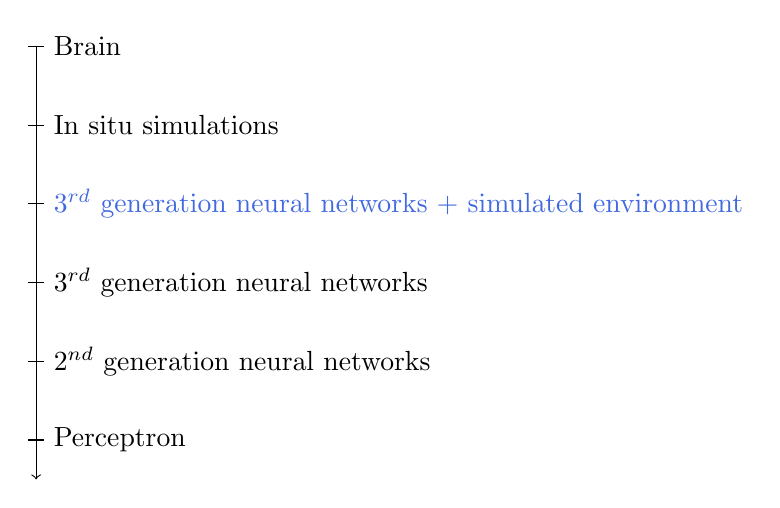
\begin{tikzpicture}
    \draw[<-] (0, -0.5) -- (0, 5);
    \draw (-0.1, 5) -- (0.1, 5) node[right] {Brain};
    \draw (-0.1, 4) -- (0.1, 4) node[right] {In situ simulations};
    \draw (-0.1, 3) -- (0.1, 3) node[right] {\color{RoyalBlue}$3^{rd}$ generation neural networks + simulated environment};
    \draw (-0.1, 2) -- (0.1, 2) node[right] {$3^{rd}$ generation neural networks};
    \draw (-0.1, 1) -- (0.1, 1) node[right] {$2^{nd}$ generation neural networks};
    \draw (-0.1, 0) -- (0.1, 0) node[right] {Perceptron};
\end{tikzpicture}

\subsection{Bodies and their environment}
In our only role model for General Intelligence, the human brain, a separation of the mind and
the body it is residing in is unfeasable~\cite{Dudai2014}. If we believe that nature is a good 
indicator for the necessary attributes of General Intelligence, the concequent thing to do is not 
abstract away the bodily environment and its steering needs that gave rise to the mind in the first place~\cite{Jekely2010}. 
A simulation capable of producing AGI must therefore in our opinion contain not only ``brains in jars'', but 
also provide a body with which a simulated organism can interact with other organisms in a social manner and a 
sandbox-like environment that is susceptible to change.
But how far should such a simulation go? Which attributes of the real world are worth simulating in a way 
that contributes to the emergence of AGI\@?

\subsection{Social interaction}
The human brain does not only thrive on sensory input, it
\emph{demands} interaction. Deprived of these stimulations,
the brain suffers damage and enforces sensory feedback by employing
hallucinations~\cite{Grassian2006}. From this, we can infer that
our simulation must provide organisms with information about their surroundings.
This includes the ability to communicate with other organisms over some
kind of arbitrary protocol. By emiting own messages over the protocol and
rewarding organisms that adhere to instructions broadcasted in this manner,
we can steer how the organisms interpret and shape this common ``language''.

\subsection{Life-sustaining ressources}
In order to encourage neuroplasticity and adaptivity, the organisms should be 
forced out of their comfort zone, as they could stagnate otherwise.
To achieve this, the environment continuously alters itself to shift its ressources.
Another great booster of evolution is competition in a predator-prey environment~\cite{Dawkins1982}.
Both of these concepts can be described in nature as a concequence of the need for ressources 
used in building survival machines, in Dawkin's words. 
By introducing the idea of depleting ressources in organisms that are necessary for survival, 
i.e. \emph{energy}, we can guide their behaviour by placing objects inside the world which organisms can consume
in order to regain energy. The initial energy sources conceived by us are \emph{plants} and \emph{water}.

\subsection{Training}
The driving force behind evolution is the gene seeking immortality~\cite{Dawkins1976}.
As conventional training with backpropagation proves to be impractical when used with
spiking neural networks~\cite{Paugam-Moisy2012}, genetic algorithms seem like a natural training choice
when going for a nature-inspired simulation. Additionaly, it is our belief that the clear error
coefficient used in backpropagation is an unrealistic ideal and, by virtue of being calculated for
a specific task, contributes to the aforementioned lack of plasticity in second-generation neural networks.

As we want to train our AI to aquire general skills, the function governing the reproductive success of
the organisms for the genetic algorithm has to be general as well. The most general reward system
is one that does not reward anything specific at all. The organism that spreads its 
genes is not determined by a hard-coded reward system, but by the organism's ability to reproduce, 
just like in real life. This way, we shift the burden of defining what is considered ``good fitness''
away from a pre-defined algorithm into the fabric of the simulation itself.
For this, we propose giving the organisms the ability to consent to sexual reproduction.
